In this section, we discuss the performance of \pred\ against the other baselines in the bilinear setting. 
%
%
Again note that the number of tasks $\Mpr \gg A \geq n$.
%
% Finally recall that when the horizon is small the weak demonstrator $\pi^w$ does not have sufficient samples for each action. This leads to a poor approximation of the greedy action. 
%
Through this experiment, we want to evaluate the performance of \pred\ to exploit the underlying latent structure and reward correlation when the horizon is small, the number of tasks is large, and understand its performance in the bilinear bandit setting \citep{jun2019bilinear, lu2021low, kang2022efficient, mukherjee2023multi}.
%
Note that this setting also goes beyond the linear feedback model \citep{abbasi2011improved, lattimore2020bandit} and is related to matrix bandits \citep{yang2020reinforcement}.


\textbf{Bilinear bandit setting:} In the bilinear bandits the learner is provided with two sets of action sets, $\X\subseteq\R^{d_1}$ and $\Z\subseteq\R^{d_2}$ which are referred to as the left and right action sets. At every round $t$ the learner chooses a pair of actions $\bx_t\in\X$ and $\bz_t\in\Z$ and observes a reward 
\begin{align*}
    r_t = \bx_t^\top \bTheta_* \bz_t + \eta_t
\end{align*}
where $\bTheta_*\in\R^{d_1\times d_2}$ is the unknown hidden matrix which is also low-rank. The $\eta_t$ is a $\sigma^2$ sub-Gaussian noise. In the multi-task bilinear bandit setting we now have a set of $M$ tasks where the reward for the $m$-th task at round $t$ is given by
\begin{align*}
    r_{m,t} = \bx_{m,t}^\top \bTheta_{m,*} \bz_{m,t} + \eta_{m,t}.
\end{align*}
Here  $\bTheta_{m,*}\in\R^{d_1\times d_2}$ is the unknown hidden matrix for each task $m$, which is also low-rank. The $\eta_{m,t}$ is a $\sigma^2$ sub-Gaussian noise. Let $\kappa$ be the rank of each of these matrices $\bTheta_{m, *}$.

A special case is the rank $1$ structure where $\bTheta_{m, *} = \btheta_{m,*}\btheta_{m,*}^\top$ where $\bTheta_{m,*} \in \R^{d \times d}$ and $\btheta_{m,*}\in\R^d$ for each task $m$. Let the left and right action sets be also same such that $\bx_{m,t} \in \X \subseteq \R^{d}$. Observe then that the reward for the $m$-th task at round $t$ is given by
\begin{align*}
    r_{m,t} = \bx_{m,t}^\top \bTheta_{m,*} \bx_{m,t} + \eta_{m,t} = (\bx_{m,t}^\top\btheta_{m, *})^2 + \eta_{m,t}.
\end{align*}
This special case is studied in \citet{chaudhuri2017active}.

\textbf{Baselines:} We again implement the same baselines discussed in \Cref{sec:short-horizon}. The baselines are \pred, \predt, \dptg, and \ts. 
%
Note that we do not implement the \linucb\ and \mlin\ for the bilinear bandit setting.
%
However, we now implement the \estr\ \citep{jun2019bilinear} which is optimal in the bilinear bandit setting. 


\textbf{\estr:} The \estr\ algorithm first estimates the unknown parameter $\bTheta_{m,*}$ for each task $m$ using E-optimal design \citep{pukelsheim2006optimal, fedorov2013theory, jun2019bilinear} for $n_1$ rounds. Let $\wTheta_{m,n_1}$ be the estimate of $\bTheta_{m,*}$ at the end of $n_1$ rounds. Let the SVD of $\wTheta_{m,n_1}$ be given by $\operatorname{SVD}(\wTheta_{m,n_1}) = \wU_{m,n_1}\widehat{\mathbf{S}}_{m, n_1}\wV_{m, n_1}$.
%
Then \estr\ rotates the actions as follows:
\begin{align*}
    \X^{\prime}_m=\left\{\left[\wU_{m,n_1} \wU^{\perp}_{m,n_1}\right]^{\top} \bx_m: \bx_m \in \X\right\} \textbf{ and } \Z^{\prime}=\left\{\left[\wV_{m,n_1} \wV^{\perp}_{m,n_1}\right]^{\top} \bz_m: \bz_m \in \Z\right\}.
\end{align*}
Then defines a vectorized action set for each task $m$ so that the last $\left(d_1-\kappa\right) \cdot\left(d_2-\kappa\right)$ components are from the complementary subspaces:
\begin{align*}
\widetilde{\A}_m&=\left\{\left[\operatorname{vec}\left(\bx_{m, 1: \kappa} \bz_{m, 1: \kappa}^{\top}\right) ; \operatorname{vec}\left(\bx_{m, \kappa+1: d_1} \bz_{m, 1: \kappa}^{\top}\right) ; \operatorname{vec}\left(\bx_{m, 1: \kappa} \bz_{m, \kappa+1: d_2}^{\top}\right) ; \right.\right.\\
%%%%%%%%%%%%%%%%
&\quad\quad\left.\left.\operatorname{vec}\left(\bx_{m, \kappa+1: d_1} \bz_{m, \kappa+1: d_2}^{\top}\right)\right] \in \mathbb{R}^{d_1 d_2}: \bx_m \in \X^{\prime}_m, \bz_m \in \Z^{\prime}_m\right\} .
\end{align*}
%
Finally for $n_2=n-n_1$ rounds, \estr\ invokes the specialized OFUL algorithm \citep{abbasi2011improved}  for the rotated action set $\widetilde{\A}_m$ with the low dimension $k=\left(d_1+d_2\right) \kappa-\kappa^2$.
% , and $\gamma\left(T_1\right)$
%
Note that the \estr\ runs the per-task low dimensional OFUL algorithm rather than learning the underlying structure across the tasks \citep{mukherjee2023multi}. 

\textbf{Outcomes:} We first discuss the main outcomes of our experimental results for increasing the horizon:

% \noindent
% \textbf{(1)} The \pred\ (\gt) learns to exploit the underlying latent bilinear structure and reward correlation between the different tasks even when $A \geq n$ but $\Mpr \gg A$.

% \textbf{(2)} The \pred\ (\gt) has lower regret than its weak demonstrator \ts\ which does not know the underlying bilinear structure.

% \textbf{(3)} The \pred\ (\gt) has lower regret compared to \dptg\ and \ad. Also, observe that \pred\ matches the performance of \estr.

\begin{tcolorbox}
\customfinding \pred\ (\gt) outperforms \dptg, \ad, and matches the performance of \estr\ in bilinear bandit setting. 
\end{tcolorbox}


% \begin{figure}[!hbt]
% \centering
% \begin{tabular}{cc}
% %%%%%%%%%%
% \hspace*{-1.5em}\subfigure[Rank $1$ $\bTheta_{m, *}$]{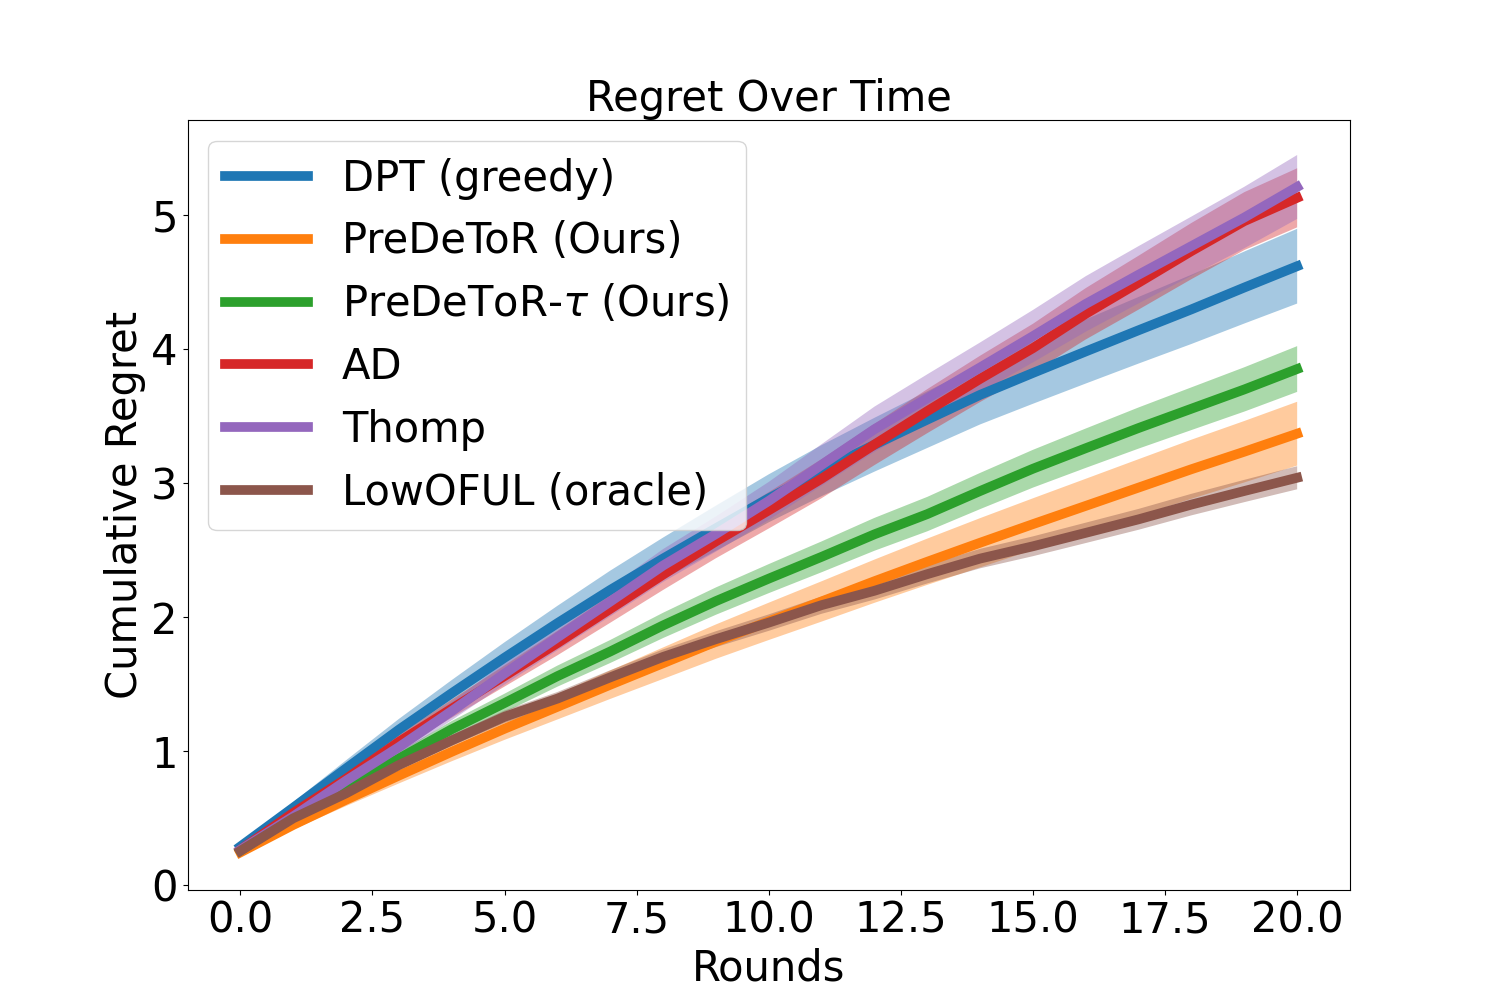
\includegraphics[scale = 0.15]{img/Neurips/bilinear/bilin_1_lr0.00015_do0_embd32_layer4_head4_envs200019_hists1_samples1_var0.3_cov0.0_H21_d20_lind3_seed1_testcov0.0_hor21.pkl.png} \label{fig:bilin-1}} &
% %%%%%%%%%%%%%%%%%%%%%%%%%%%%%%%
% \hspace*{-1.5em}\subfigure[Rank $2$ $\bTheta_{m, *}$]{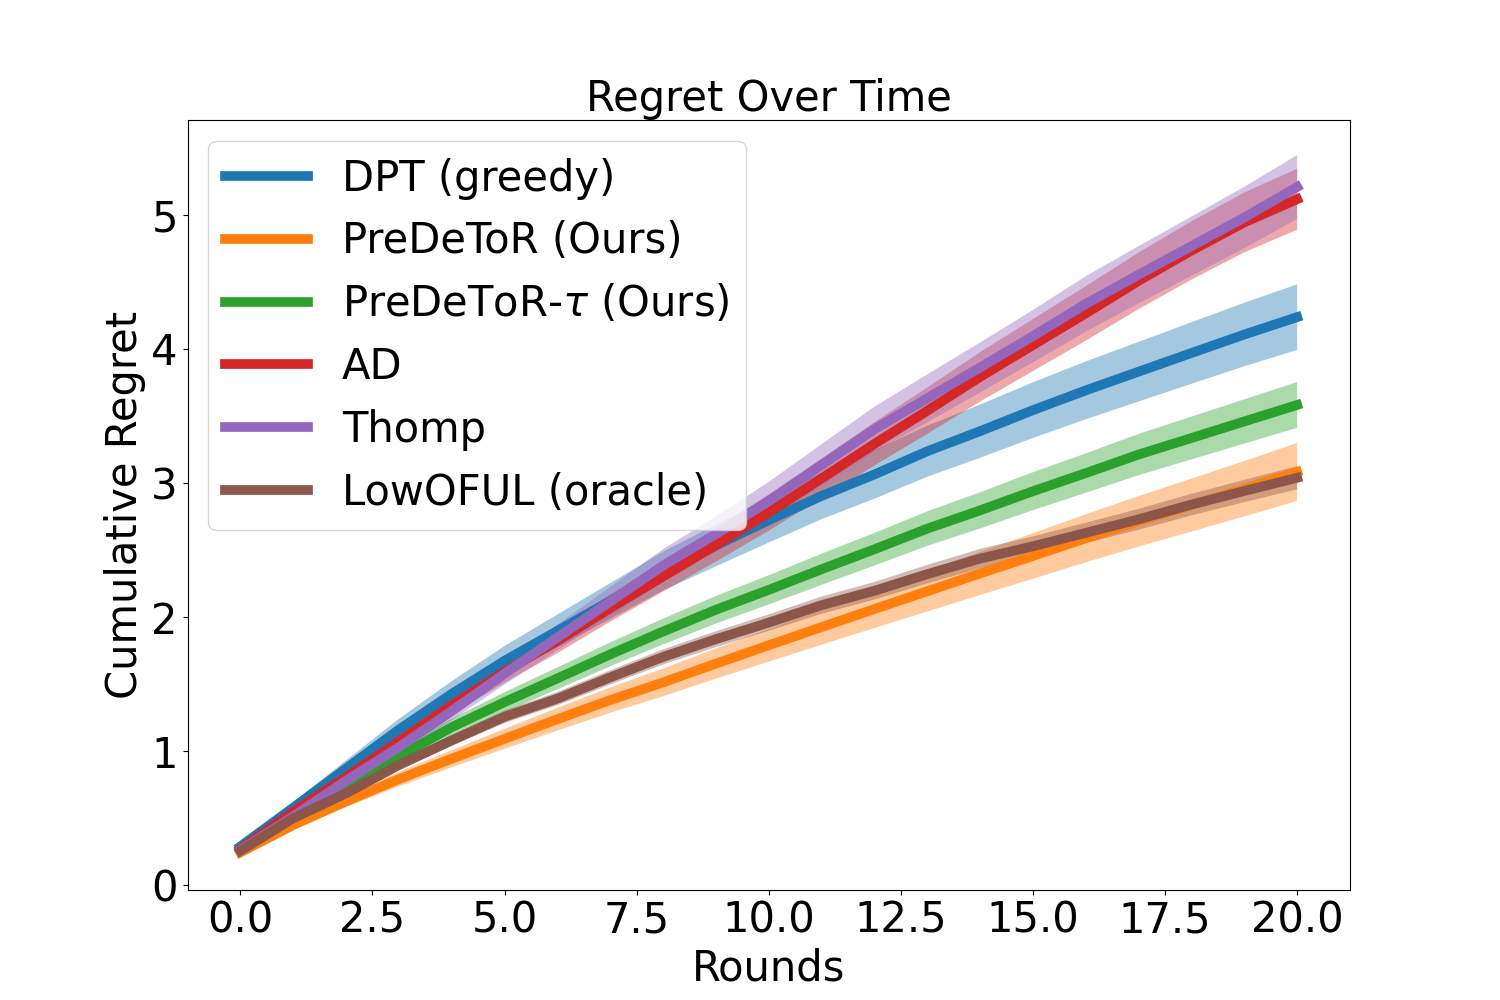
\includegraphics[scale = 0.15]{img/Neurips/bilinear/bilin_2_lr0.00015_do0_embd32_layer4_head4_envs250029_hists1_samples1_var0.3_cov0.0_H21_d20_lind3_seed1_testcov0.0_hor21.pkl.png} \label{fig:bilin-2}}
% \end{tabular}
% \vspace*{-1em}
% \caption{Experiment with bilinear bandits. The y-axis shows the cumulative regret.}
% \label{fig:expt-bilin}
% \end{figure}

\begin{figure}[!hbt]
\centering
\begin{subfigure}[b]{0.48\textwidth}
    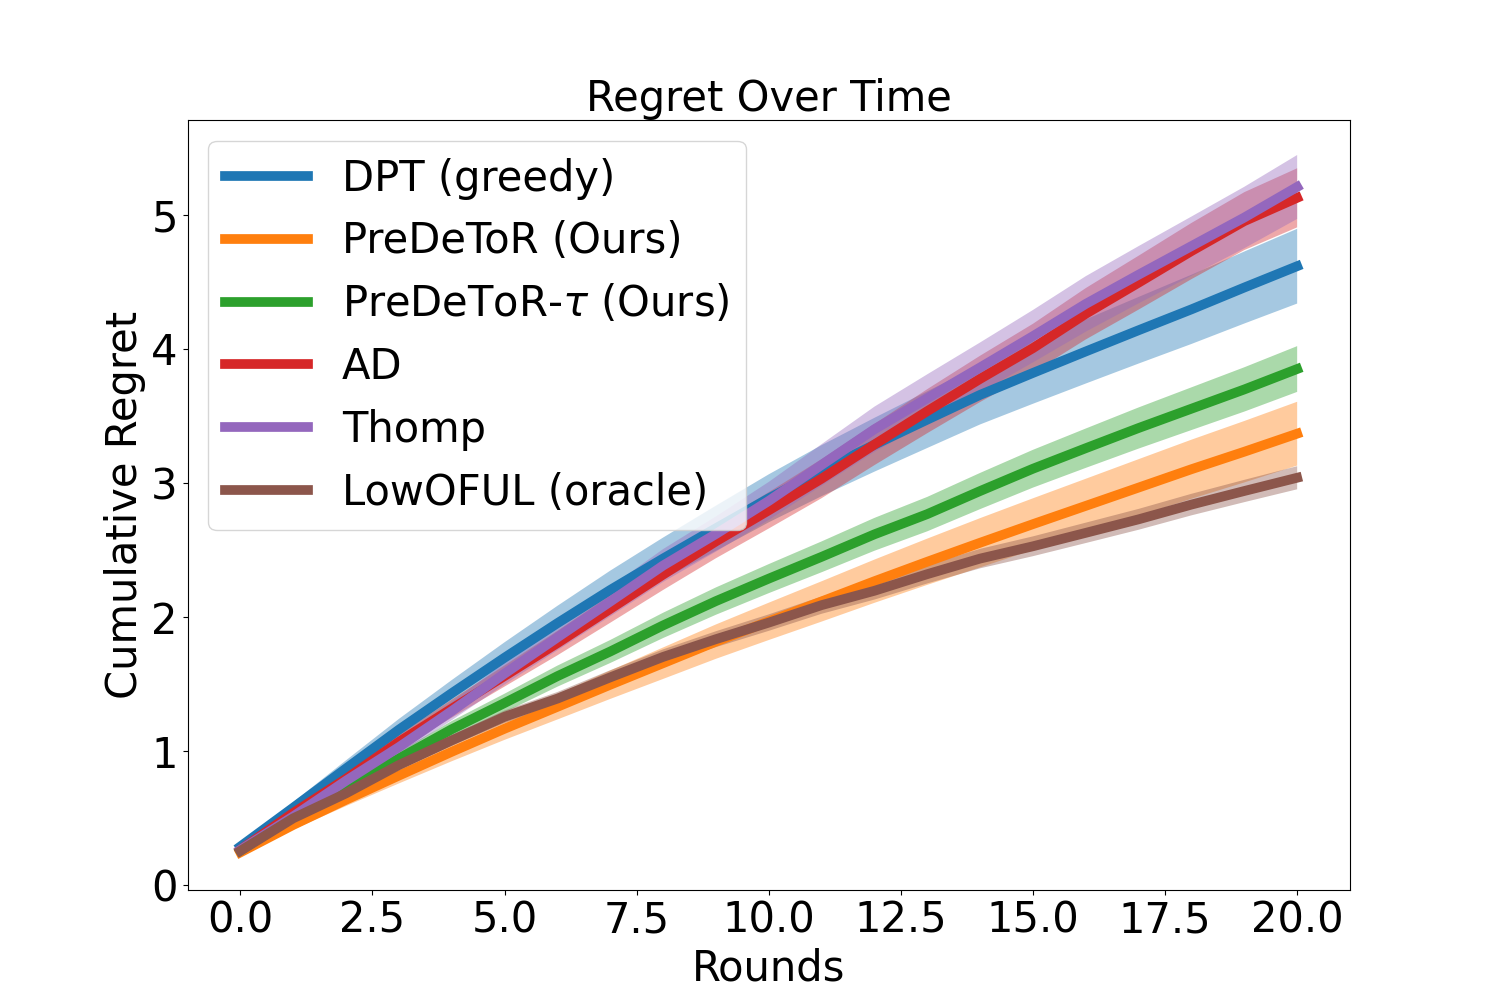
\includegraphics[scale=0.15]{img/Neurips/bilinear/bilin_1_lr0.00015_do0_embd32_layer4_head4_envs200019_hists1_samples1_var0.3_cov0.0_H21_d20_lind3_seed1_testcov0.0_hor21.pkl.png}
    \caption{Rank $1$ $\bTheta_{m, *}$}
    \label{fig:bilin-1}
\end{subfigure}%
\begin{subfigure}[b]{0.48\textwidth}
    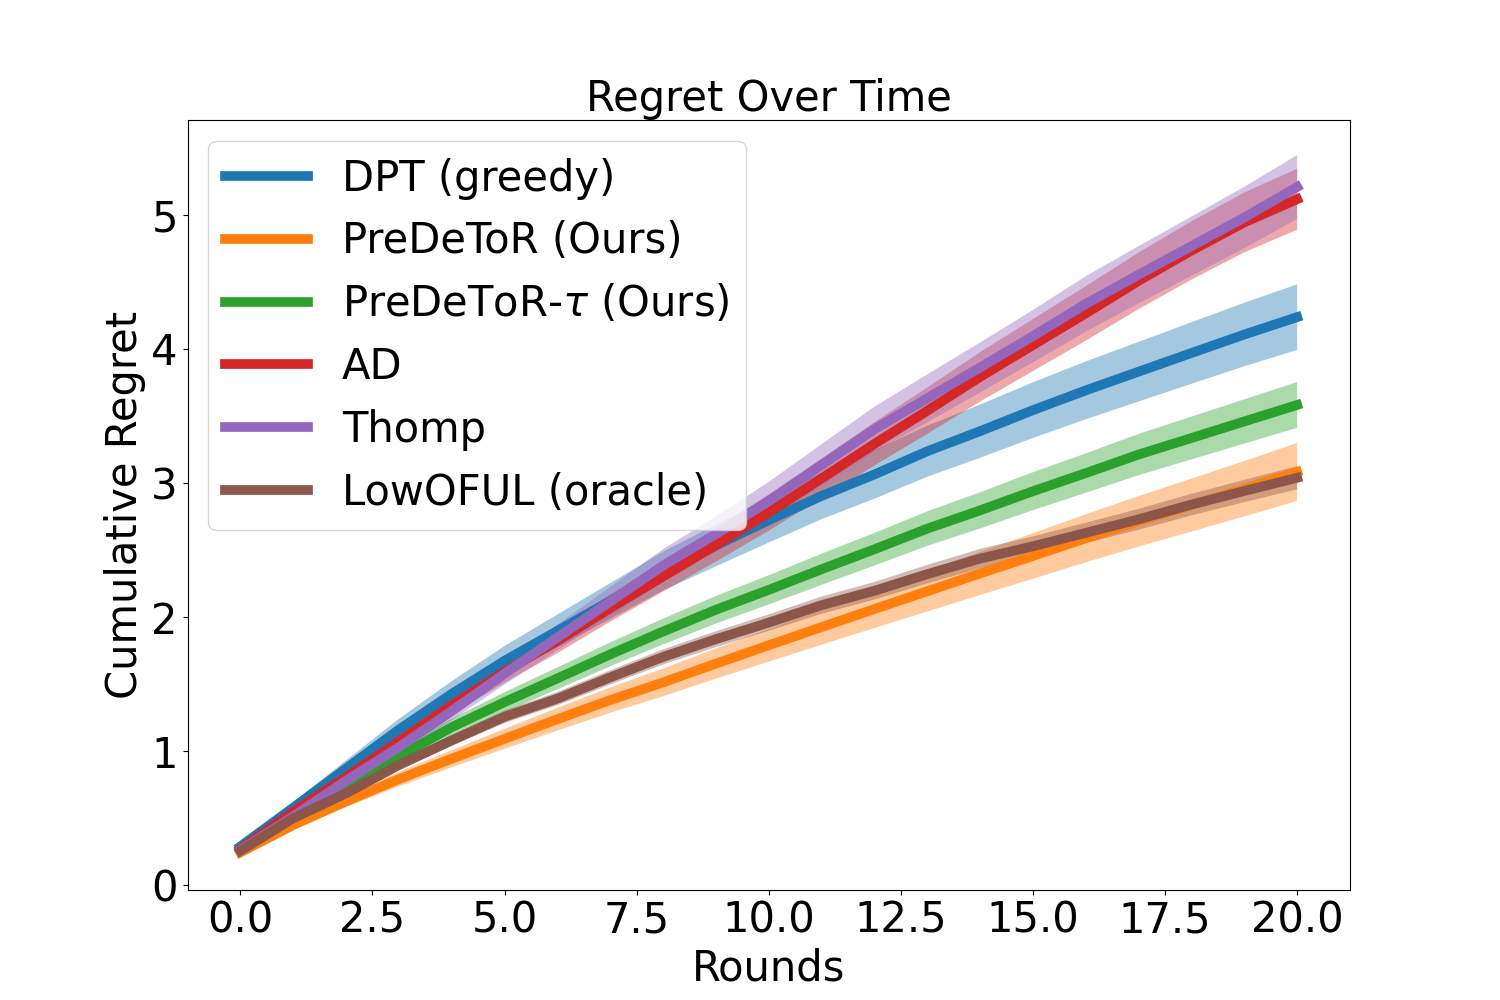
\includegraphics[scale=0.15]{img/Neurips/bilinear/bilin_2_lr0.00015_do0_embd32_layer4_head4_envs250029_hists1_samples1_var0.3_cov0.0_H21_d20_lind3_seed1_testcov0.0_hor21.pkl.png}
    \caption{Rank $2$ $\bTheta_{m, *}$}
    \label{fig:bilin-2}
\end{subfigure}
\vspace*{-1em}
\caption{Experiment with bilinear bandits. The y-axis shows the cumulative regret.}
\label{fig:expt-bilin}
\end{figure}

\textbf{Experimental Result:} We observe these outcomes in \Cref{fig:expt-bilin}. In \Cref{fig:bilin-1} we experiment with rank $1$ hidden parameter $\bTheta_{m,*}$ and set horizon $n=20$, $\Mpr =  200000$, $\Mts = 200$, $A=30$, and $d=5$. 
%
In \Cref{fig:bilin-2} we experiment with rank $2$ hidden parameter $\bTheta_{m,*}$ and set horizon $n=20$, $\Mpr =  250000$, $\Mts = 200$, $A=25$, and $d=5$. 
%
%
Again, the demonstrator $\pi^w$ is the \ts\ algorithm. We observe that \pred\ has lower cumulative regret than \dptg, \ad\ and \ts. Note that for any task $m$ for the horizon $20$ the \ts\ will be able to sample all the actions at most once.
% Moreover \pred\ matches the performance of \linucb. 
%
%The weak performance of \dptg\ can be attributed to both short horizons and the inability to estimate the optimal action for such a short horizon $H < A$. 
%
Note that for this small horizon setting the \dptg\ does not have a good estimation of $\widehat{a}_{m,*}$ which results in a poor prediction of optimal action $\widehat{a}_{m,t,*}$. In contrast \pred\ learns the correlation of rewards across tasks and can perform well.
% This results in higher regret. 
Observe from \Cref{fig:bilin-1}, and \ref{fig:bilin-2} that \pred\ has lower regret than \ts\ and matches \estr. Also, in this low-data regime it is not enough for \estr\ to learn the underlying $\bTheta_{m, *}$ with high precision. Hence, \pred\ also has slightly lower regret than \estr. 
%
% The training of \ad\ ensures that it does not outperform the demonstrator \ts.
Note that the main objective of \ad\ is to match the performance of its demonstrator.
%
Most importantly it shows that \pred\ can exploit the underlying latent structure and reward correlation better than \dptg, and \ad.
